\documentclass[a4paper, 11pt, oneside]{article}

\usepackage[utf8]{inputenc}
\usepackage[T1]{fontenc}
\usepackage[french]{babel}
\usepackage{array}
\usepackage{shortvrb}
\usepackage[fleqn]{amsmath}
\usepackage{amsfonts}
\usepackage{fullpage}
\usepackage{enumerate}
\usepackage{graphicx}            
\usepackage{subfigure}      
\usepackage{alltt}
\usepackage{url}
\usepackage{indentfirst}
\usepackage{eurosym}
\usepackage{listings}
\usepackage{color}
\usepackage[table,xcdraw,dvipsnames]{xcolor}
\usepackage{multirow}
\usepackage{float}

\definecolor{mygray}{rgb}{0.5,0.5,0.5}
\newcommand{\coms}[1]{\textcolor{MidnightBlue}{#1}}

\lstset{
    language=C, % Utilisation du langage C
    commentstyle={\color{MidnightBlue}}, % Couleur des commentaires
    frame=single, % Entoure le code d'un joli cadre
    rulecolor=\color{black}, % Couleur de la ligne qui forme le cadre
    stringstyle=\color{RawSienna}, % Couleur des chaines de caractères
    numbers=left, % Ajoute une numérotation des lignes à gauche
    numbersep=5pt, % Distance entre les numérots de lignes et le code
    numberstyle=\tiny\color{mygray}, % Couleur des numéros de lignes
    basicstyle=\tt\footnotesize,
    tabsize=3, % Largeur des tabulations par défaut
    keywordstyle=\tt\bf\footnotesize\color{Sepia}, % Style des mots-clés
    extendedchars=true,
    captionpos=b, % sets the caption-position to bottom
    texcl=true, % Commentaires sur une ligne interprétés en Latex
    showstringspaces=false, % Ne montre pas les espace dans les chaines de caractères
    escapeinside={(>}{<)}, % Permet de mettre du latex entre des <( et )>.
    inputencoding=utf8,
    literate=
  {á}{{\'a}}1 {é}{{\'e}}1 {í}{{\'i}}1 {ó}{{\'o}}1 {ú}{{\'u}}1
  {Á}{{\'A}}1 {É}{{\'E}}1 {Í}{{\'I}}1 {Ó}{{\'O}}1 {Ú}{{\'U}}1
  {à}{{\`a}}1 {è}{{\`e}}1 {ì}{{\`i}}1 {ò}{{\`o}}1 {ù}{{\`u}}1
  {À}{{\`A}}1 {È}{{\`E}}1 {Ì}{{\`I}}1 {Ò}{{\`O}}1 {Ù}{{\`U}}1
  {ä}{{\"a}}1 {ë}{{\"e}}1 {ï}{{\"i}}1 {ö}{{\"o}}1 {ü}{{\"u}}1
  {Ä}{{\"A}}1 {Ë}{{\"E}}1 {Ï}{{\"I}}1 {Ö}{{\"O}}1 {Ü}{{\"U}}1
  {â}{{\^a}}1 {ê}{{\^e}}1 {î}{{\^i}}1 {ô}{{\^o}}1 {û}{{\^u}}1
  {Â}{{\^A}}1 {Ê}{{\^E}}1 {Î}{{\^I}}1 {Ô}{{\^O}}1 {Û}{{\^U}}1
  {œ}{{\oe}}1 {Œ}{{\OE}}1 {æ}{{\ae}}1 {Æ}{{\AE}}1 {ß}{{\ss}}1
  {ű}{{\H{u}}}1 {Ű}{{\H{U}}}1 {ő}{{\H{o}}}1 {Ő}{{\H{O}}}1
  {ç}{{\c c}}1 {Ç}{{\c C}}1 {ø}{{\o}}1 {å}{{\r a}}1 {Å}{{\r A}}1
  {€}{{\euro}}1 {£}{{\pounds}}1 {«}{{\guillemotleft}}1
  {»}{{\guillemotright}}1 {ñ}{{\~n}}1 {Ñ}{{\~N}}1 {¿}{{?`}}1
}
\newcommand{\tablemat}{~}


\newcommand{\intitule}{INFO0030 : Projet 4 - Five or More}
 \newcommand{\GrNbr}{03}
 \newcommand{\PrenomUN}{Sami}
 \newcommand{\NomUN}{Ouazouz}
 \newcommand{\PrenomDEUX}{Muhammad}
 \newcommand{\NomDEUX}{Qayyum}

\renewcommand{\tablemat}{\tableofcontents}


\title{INFO0947: \intitule}
\author{Groupe \GrNbr : \PrenomUN~\textsc{\NomUN}, \PrenomDEUX~\textsc{\NomDEUX}}
\date{}
\begin{document}

\maketitle
\newpage
\tablemat
\newpage

%%%%%%%%%%%%%%%% RAPPORT %%%%%%%%%%%%%%%

\section{Introduction}\label{introduction}

Ce projet consistait à développer une implémentation du jeu "Five or More", 
où le joueur doit déplacer des boules de différentes couleurs sur une grille en créant des 
alignements d'au moins cinq boules de même couleur, générant ainsi du score. 
Notre travail a porté sur la conception d'une interface graphique 
utilisant la bibliothèque GTK2+, ainsi que sur l'implémentation de la logique 
de jeu en langage C avec divers algorithmes.

\section{Architecture générale du code}\label{architecture}

Notre implémentation suit le modèle d'architecture MVC (Modèle-Vue-Contrôleur) pour structurer clairement notre code et séparer les différentes préoccupations:

\begin{itemize}
    \item \textbf{Modèle} (\texttt{modele.h}, \texttt{modele.c}): Contient les structures de données fondamentales du jeu (plateau, cases, scores) et les fonctions pour y accéder et les manipuler. Le modèle implémente la logique de base du jeu comme la vérification des alignements et la gestion des scores.
    
    \item \textbf{Vue} (\texttt{vue.h}, \texttt{vue.c}): Gère tout ce qui touche à l'interface graphique, depuis la création des fenêtres et boutons jusqu'aux dialogues et à l'affichage du jeu. La vue n'a aucune connaissance de la logique de jeu elle-même.
    
    \item \textbf{Contrôleur} (\texttt{controle.h}, \texttt{controle.c}): Fait le lien entre le modèle et la vue. Il traite les événements utilisateur (clics sur les boutons, sélections dans les menus) et met à jour le modèle et la vue en conséquence.
    
    \item \textbf{Utilitaires} (\texttt{utilis.h}, \texttt{utilis.c}): Contient des fonctions d'assistance qui ne relèvent pas strictement d'un des trois composants principaux, comme des fonctions de gestion d'images et des générateurs de boules.
\end{itemize}

Cette architecture a permis une séparation claire des responsabilités et a facilité le développement parallèle par les membres de l'équipe.



\section{Structures de données}\label{structures}

\subsection{Structures principales}

Nous avons conçu plusieurs structures de données opaques pour encapsuler les éléments du jeu. Voici leurs définitions complètes:

\begin{lstlisting}[language=C, caption=Structure Plateau\_t]
/**
 * @struct Plateau_t
 * @brief Structure principale representant le plateau de jeu
 */
typedef struct Plateau_t {
    int largeur;              // Nombre de colonnes
    int hauteur;              // Nombre de lignes
    int nb_types_symboles;    // Nombre de couleurs differentes
    int symboles_par_tour;    // Nombre de boules par tour
    int nb_cases_remplies;    // Nombre de cases occupees
    Case **cases;             // Tableau 2D des cases du plateau
    int difficulte;           // Niveau de difficulte
    Score score;              // Score actuel
    int nb_suivantes;         // Nombre de boules suivantes
    Couleur boules_suivantes[MAX_SUIVANTS];// Tableau des couleurs des boules suivantes
    GtkWidget **boutons_suivants;  // Boutons representant les boules suivantes
} Plateau;
\end{lstlisting}

\begin{lstlisting}[language=C, caption=Structure Case\_t]
/**
 * @struct Case_t
 * @brief Structure representant une case du plateau de jeu
 */
typedef struct Case_t {
    bool occupe;       // Indique si la case contient une boule
    Couleur col;       // Couleur de la boule (si presente)
    GtkWidget *image;  // Bouton GTK representant la case
} Case;
\end{lstlisting}

\begin{lstlisting}[language=C, caption=Structure Score\_t]
/**
 * @struct Score_t
 * @brief Structure representant un score dans le jeu
 */
typedef struct Score_t {
    char nom[MAX_NOM + 1];  // Nom du joueur
    int valeur;             // Valeur du score
} Score;
\end{lstlisting}

\begin{lstlisting}[language=C, caption=Structure Boule\_t]
/**
 * @struct Boule_t
 * @brief Structure representant une boule
 */
typedef struct Boule_t {
    Couleur couleur;    // Couleur de la boule
    GtkWidget *image;   // Image associee a la boule
} Boule;
\end{lstlisting}

\subsection{Structures auxiliaires}

En plus des structures principales, nous utilisons des structures auxiliaires pour faciliter certaines opérations:

\begin{lstlisting}[language=C, caption=Structure MiseAJour]
/**
 * @brief Structure utilisee pour la mise a jour des cases 
 * et la recherche de boutons
 */
typedef struct {
    int ligne_actuelle;      // Coordonnee ligne de la case recherchee
    int colonne_actuelle;    // Coordonnee colonne de la case recherchee
    Plateau *plateau;        // Plateau de jeu concerne
    GtkWidget *est_bouton;   // Bouton trouve
    GtkWidget *bouton_trouve;// Bouton trouve (alternative)
} MiseAJour;
\end{lstlisting}

\begin{lstlisting}[language=C, caption=Structure Data]
/**
 * @brief Structure utilisee pour les recherches de widgets dans l'interface
 */
typedef struct {
    GtkWidget *est_widget;   // Widget trouve
    gboolean est_trouve;     // Indique si un widget a ete trouve
} Data;
\end{lstlisting}

\begin{lstlisting}[language=C, caption=Structure InfosCallback]
   /**
    * @brief Structure utilisee pour stocker des informations dans les callbacks
    */
   typedef struct {
       int ligne_actuelle;      // Coordonnee ligne de la case courante
       int colonne_actuelle;    // Coordonnee colonne de la case courante
       Plateau *plateau;        // Plateau de jeu concerne
   } InfosCallback;
   \end{lstlisting}

\section{Algorithmes particuliers}\label{algorithmes}

\subsection{Algorithme de recherche de chemin}

L'un des algorithmes les plus importants de notre jeu est la recherche de chemin entre deux cases, pour déterminer si un déplacement de boule est possible. Nous avons implémenté un algorithme de parcours en largeur (BFS) qui:

\begin{itemize}
    \item Utilise une file (avec GQueue de GLib) pour stocker les cases à explorer
    \item Maintient une matrice \texttt{visited} pour marquer les cases déjà visitées
    \item Explore les cases adjacentes (haut, bas, gauche, droite) tant qu'elles sont libres
    \item S'arrête dès que la case d'arrivée est atteinte, ou quand toutes les possibilités sont épuisées
\end{itemize}

La complexité temporelle de cet algorithme est $O(n \times m)$ dans le pire des cas, où $n$ et $m$ sont les dimensions du plateau. Cette complexité est optimale car, dans le pire cas, il peut être nécessaire d'explorer toutes les cases du plateau.

\subsection{Algorithme de vérification des alignements}

Un autre algorithme clé est celui qui vérifie s'il existe des alignements d'au moins cinq boules de même couleur. Notre implémentation:

\begin{itemize}
    \item Parcourt le plateau en vérifiant les quatre directions possibles 
    pour chaque case: horizontale, verticale, et les deux diagonales
    \item Pour chaque direction, compte le nombre de boules consécutives de même couleur
    \item Si un alignement d'au moins cinq boules est trouvé, marque ces cases 
    pour suppression et ajoute des points au score. Pour supprimer les cases, 
    on a décidé d'allouer de la mémoire un tableau.
    \item La suppression effective est réalisée dans un second passage
     pour éviter des problèmes de comptage
\end{itemize}

La complexité temporelle de cet algorithme est $O(n \times m \times 4)$, soit $O(n \times m)$, 
car pour chaque case, nous vérifions dans les quatre directions possibles.


\section{Gestion du code}\label{gestion}

Dans le cadre de ce projet, nous avons utilisé \textbf{GitLab} comme système de 
gestion de versions (SCM - \textit{Source Control Management}). Cet outil nous 
a permis de collaborer efficacement à plusieurs sur le même dépôt de code, 
tout en assurant un suivi structuré des modifications apportées au fil du temps.
Voici le lien vers notre dépôt : \url{https://gitlab.uliege.be/Muhammad.Qayyum/info0030_groupe03.git}.

Nous avons adopté une organisation basée sur trois branches principales :
\begin{itemize}
  \item \textbf{main} : la branche principale du projet, contenant le code stable et validé ;
  \item \textbf{sami} : une branche dédiée au développement du binôme Sami ;
  \item \textbf{qayyum} : une branche dédiée au développement du binôme Muhammad. \\
\end{itemize}

Cette structuration nous a permis de travailler en parallèle sans interférer 
 avec le code des autres, limitant ainsi les conflits. 
 Chaque membre développait de nouvelles fonctionnalités ou corrections 
 sur sa propre branche, avant de fusionner (merge) ses changements avec 
 la branche \textbf{main} une fois les tests validés. \\

L'utilisation de GitLab nous a également permis de suivre l'historique 
des modifications, de revenir en arrière si nécessaire 
(par exemple avec \texttt{git checkout HEAD@\{1\}} ou \texttt{git reset --hard}),
 et de gérer efficacement les conflits lors des fusions. Le contrôle de version 
 s’est avéré essentiel pour assurer la fiabilité et la continuité du 
 développement tout au long du projet.

Grâce à cet outil, nous avons pu maintenir une bonne organisation du code, 
éviter les pertes de données, et faciliter le travail collaboratif, 
même en cas de modifications simultanées.



\section{Coopération au sein du groupe}\label{cooperation}

Notre binôme a fonctionné selon une répartition des tâches basée sur nos compétences respectives:

\begin{itemize}
    \item Muhammad s'est principalement occupé de l'interface graphique et 
    de l'intégration des composants (différentes structures de données), en plus 
    de l'alogrithme permettant de vérifier les alignements.
    \item Quant à Sami, il s'est concentré sur toute la logique du jeu avec la génération 
    aléatoire des boules, le chemin possible et la gestion des scores. 
\end{itemize}

Nous avons organisé notre travail avec des réunions hebdomadaires pour faire 
le point sur l'avancement du projet. 
La communication s'est faite par des échanges réguliers sur Discord et via les issues 
et les merges sur GitLab.

Les difficultés principales que nous avons rencontrées concernaient 
l'intégration de nos parties respectives et la compréhension de certaines subtilités de GTK+. 
Nous avons résolu ces problèmes par une collaboration étroite et en consultant la documentation et les exemples vus au cours.


\section{Interface graphique}\label{interface}

Notre interface graphique est construite avec GTK+ 2.0 et s'organise de 
la manière suivante:

\begin{itemize}
    \item Une fenêtre principale contenant:
    \begin{itemize}
        \item Une barre de menu pour accéder aux fonctionnalités 
        (nouvelle partie, niveau de difficulté, scores, etc.)
        \item Une zone d'information montrant les prochaines boules et le score actuel
        \item La grille de jeu, composée de boutons représentant les cases
    \end{itemize}
\end{itemize}

\begin{figure}[H]
    \centering
    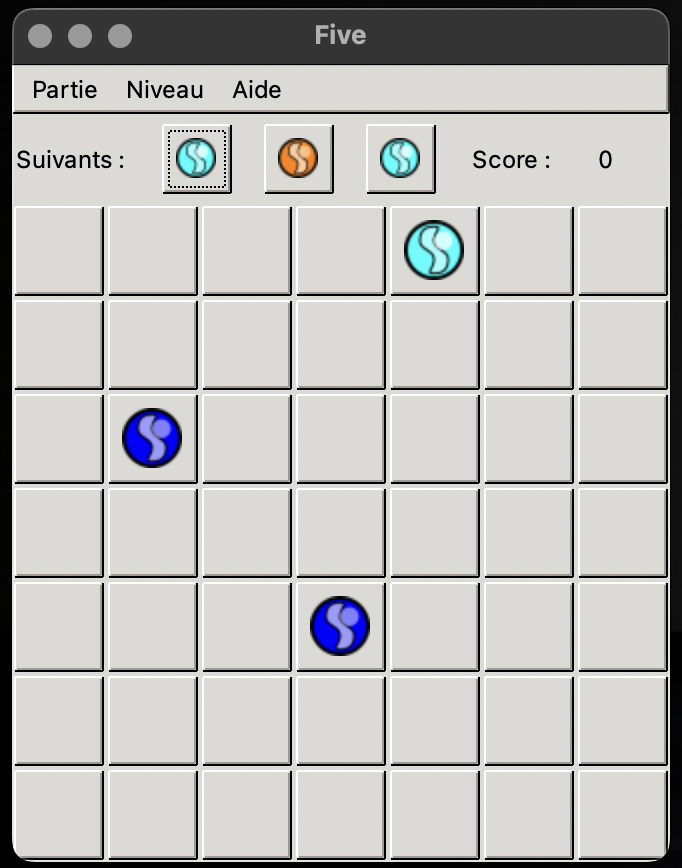
\includegraphics[width=0.4\textwidth]{interface.jpeg}
    \caption{Interface du jeu Five or More}
    \label{fig:Interface}
\end{figure}

La fenêtre est organisée avec des widgets GTK imbriqués:
\begin{itemize}
    \item La fenêtre principale contient une VBox verticale
    \item Dans cette VBox, nous avons placé:
    \begin{itemize}
        \item La barre de menu (GTK MenuBar)
        \item Une HBox horizontale pour les prochaines boules et le score
        \item Une Table GTK pour la grille de jeu, dont la taille varie selon 
        le niveau de difficulté
    \end{itemize}
\end{itemize}

Nous avons dû utiliser GtkTable pour cela. 
Chaque case du jeu est représentée par un GtkButton pouvant contenir une image 
de boule grâce à notre fonction: \\
$GtkWidget ${ }$ *charger\_image\_button(const ${ }$ char { } *chemin\_image)$


\section{Améliorations possibles}\label{ameliorations}

Si nous avions disposé d'un mois supplémentaire, plusieurs améliorations auraient été envisageables:

\begin{itemize}
    \item \textbf{Animation des déplacements}: Ajouter des animations lors du déplacement des boules pour améliorer l'expérience utilisateur.
    
    \item \textbf{Prédiction de chemin}: Afficher visuellement le chemin que la boule va emprunter lorsqu'une destination est sélectionnée.
    
    \item \textbf{Sauvegarde de partie}: Permettre d'enregistrer l'état d'une partie pour la reprendre ultérieurement avec l'ajout d'un menu.
    
    \item \textbf{Mode multijoueur}: Implémenter un mode à deux joueurs en alternance ou en compétition de score.
    
    \item \textbf{Thèmes graphiques}: Proposer différents thèmes visuels pour personnaliser l'apparence du jeu.
    
   
    \item \textbf{Optimisations}: Améliorer les performances de certains algorithmes, notamment la vérification des alignements qui pourrait être optimisée pour ne pas re-vérifier les cases déjà contrôlées.
\end{itemize}

\section{Éléments appris}\label{apprentissages}

Ce projet nous a permis d'acquérir et de renforcer plusieurs compétences:

\begin{itemize}
    \item \textbf{Programmation en C}: Approfondissement de notre maîtrise du langage C, notamment pour la gestion de la mémoire et les structures de données.
    
    \item \textbf{Programmation d'interfaces graphiques}: Découverte et pratique de la bibliothèque GTK+ pour créer des interfaces graphiques en C.
    
    \item \textbf{Architecture MVC}: Mise en pratique du pattern Modèle-Vue-Contrôleur pour structurer un projet de taille moyenne.
    
    \item \textbf{Algorithmes}: Implémentation et optimisation d'algorithmes de parcours de graphe (BFS) et de recherche de motifs.
    
    \item \textbf{Travail d'équipe}: Amélioration de nos compétences en communication, en répartition des tâches et en gestion de versions grâce à GitLab (SCM).
    
    \item \textbf{Documentation de code}: Pratique de la documentation systématique du code avec un format standardisé (Doxygen).
    
    \item \textbf{Débogage}: Développement de techniques efficaces pour identifier et résoudre les problèmes dans un code complexe.
\end{itemize}

% !TEX root = ./main.tex
%%%%%%%%%%%%%%%%%%%%%%%%%%%%%%%%%%%%%%%%%%%%%%%%%%%%%%%%%%%%%%%%%%%%%%%%%%%%%%%%%%%%%%%%%%
% Rédigez ici la conclusion de votre rapport.                                            %
%%%%%%%%%%%%%%%%%%%%%%%%%%%%%%%%%%%%%%%%%%%%%%%%%%%%%%%%%%%%%%%%%%%%%%%%%%%%%%%%%%%%%%%%%%
\section{Conclusion}\label{conclusion}
%%%%%%%%%%%%%%%%%%%%%
Pour conclure, à travers notre rapport, nous avons établi une approche
constructive pour une fonction calculant le plus long
sous-tableau qui est à la fois préfixe et suffixe d'un tableau donné. 
Nous avons défini le problème, formalisé le problème, analysé, découpé en 
sous-problèmes et avons fait une approche constructive sur la base de nos invariants.

\vspace{0.4cm}
Nous avons également calculé la complexité de notre algorithme, qui est $O(n^2)$.
Notre code peut désormais être utilisé pour résoudre le problème de manière efficace et
fiable.

\end{document}
